\documentclass[a4paper,11pt]{article}
\usepackage[T1]{fontenc}      % codifica dei font
\usepackage[utf8]{inputenc}
\usepackage[italian]{babel}
\usepackage{lipsum}
\usepackage{url}
\usepackage{amsfonts}
\usepackage{graphicx}
\begin{document}
% lettere accentate da tastiera
% lingua del documento
% genera testo fittizio
% per scrivere gli indirizzi Internet
\author{Linpeng Zhang}
\title{Tutorato AFL}
\maketitle
\begin{abstract}
    Per errori/dubbi/problemi: linpeng.zhang@studenti.unipd.it.% \\Note: 
\end{abstract}
\tableofcontents
\section{Lez3}
\subsection{Riassunto informale}
\begin{itemize}
    \item Da FA a RE, se il FA ha solo uno stato finale, basta eliminare gli stati che non sono né iniziali né finali e inserire opportune transizioni. Conviene partire da stati in cui ci sono pochi stati entranti ed uscenti;
    \item per mostrare che un linguaggio è regolare o meno si possono anche usare le proprietà di chiusura viste a lezione.
\end{itemize}
%Un automa a stati finiti, come suggerisce il nome, ha una "memoria limitata". Il mio consiglio per definire un automa che accetti un determinato linguaggio è pensare a cosa rappresenti ciascuno stato. Si noti infine che per essere sicuri che un automa riconosca un certo linguaggio bisognerebbe dimostrarlo (altrimenti non saremo mai sicuri). Ad esempio si possono dimostrare delle proprietà degli stati, o per induzione. Tuttavia, in genere, ciò non è richiesto.
\subsection{Esercizi}
    Dire se l'automa dato è deterministico; in caso contrario, definire un DFA equivalente.
    \begin{enumerate}
        \item \begin{minipage}{\linewidth}
            \centering
            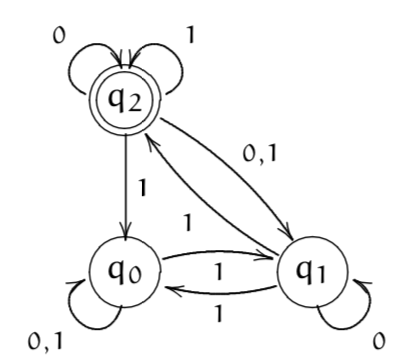
\includegraphics[width=5cm]{Fig1.png}
        \end{minipage}
    \end{enumerate}
    Costruire un FA che accetti il linguaggio denotato dalle seguenti RE:
    \begin{enumerate}
    \item $R=0^* + 1^* + (01)^*$
    \item $R=(0+1)^*1(0+1)$
    \item $R=a(a+b)^*+c$
    \end{enumerate}
    Convertire l'automa dato in una RE:
    \begin{enumerate}
        \item \begin{minipage}{\linewidth}
            \centering
            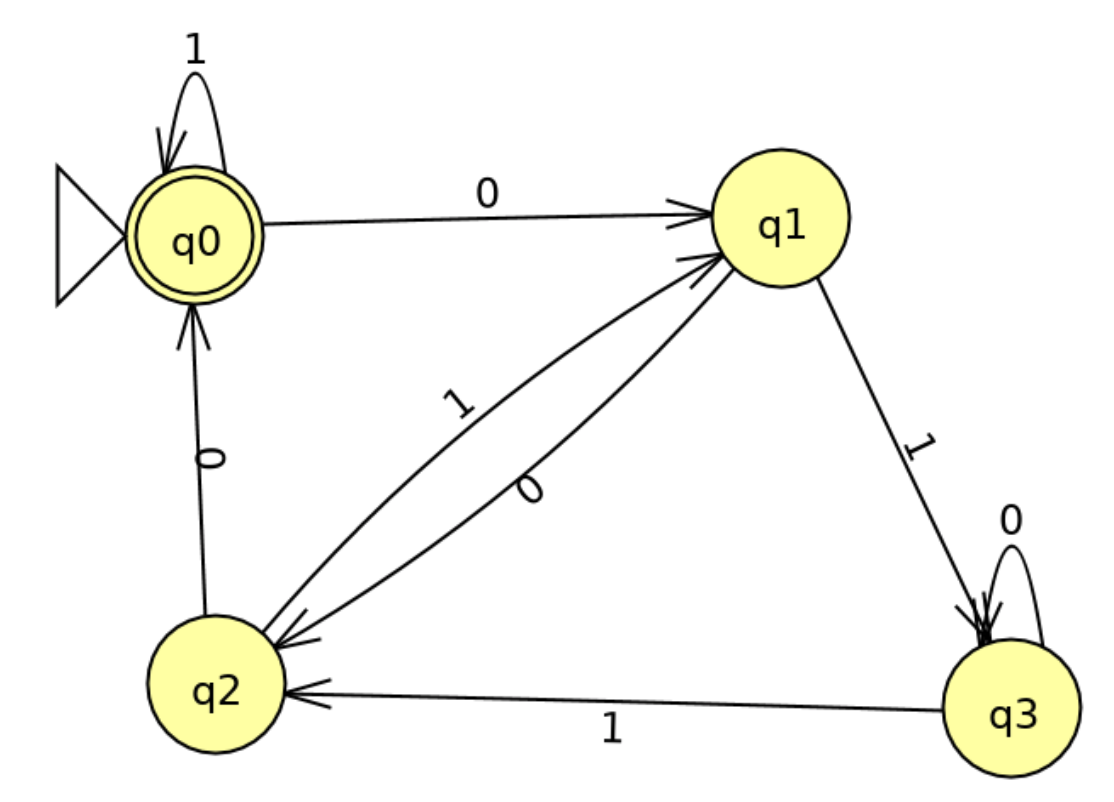
\includegraphics[width=5cm]{Lez2dfatore1.png}
        \end{minipage}
        \item \begin{minipage}{\linewidth}
                \centering
                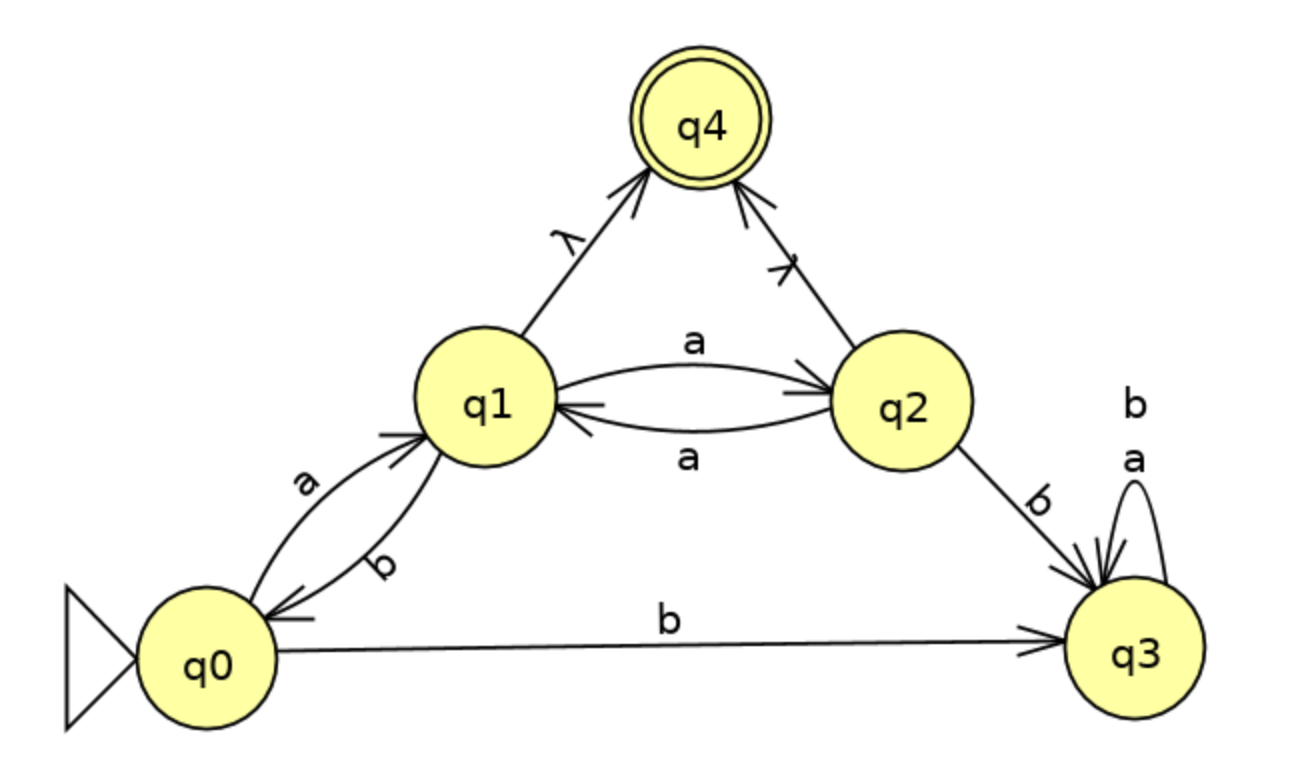
\includegraphics[width=5cm]{Lez3fatore1.png}
        \end{minipage}
    \end{enumerate}
    I seguenti linguaggi sono regolari? Motivare la risposta. 
    \begin{enumerate}
    \item $L=\{0^{5k}, k\in \mathbb{N} \}$
    \item $L=\{0^{pq},p,q\in \mathbb{N}, p>1,q>1 \}$
    \item $L=\{0^{k^3},k\in\mathbb{N} \}$
  %  \item $L=\{0^n1^m,n\neq m , n,m\in \mathbb{N}\}$
    \end{enumerate}
    \subsection{Soluzioni}
    Conversione da NFA a DFA
    \begin{enumerate}
        \item \begin{minipage}{\linewidth}
            \centering
            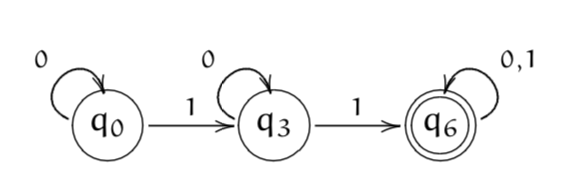
\includegraphics[width=5cm]{Lez3nfatodfa1.png}
        \end{minipage}
    \end{enumerate}
    Conversione da RE a FA
    \begin{enumerate}
        \item \begin{minipage}{\linewidth}
            \centering
            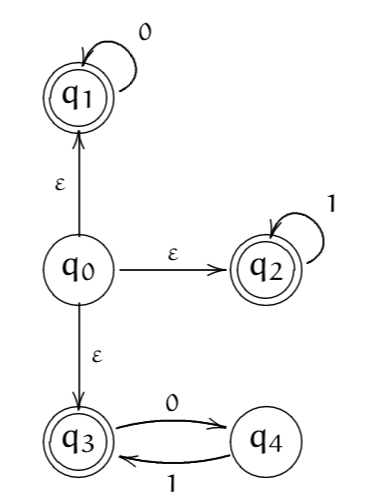
\includegraphics[width=5cm]{Lez2retodfa1.png}
        \end{minipage}
        \item \begin{minipage}{\linewidth}
            \centering
            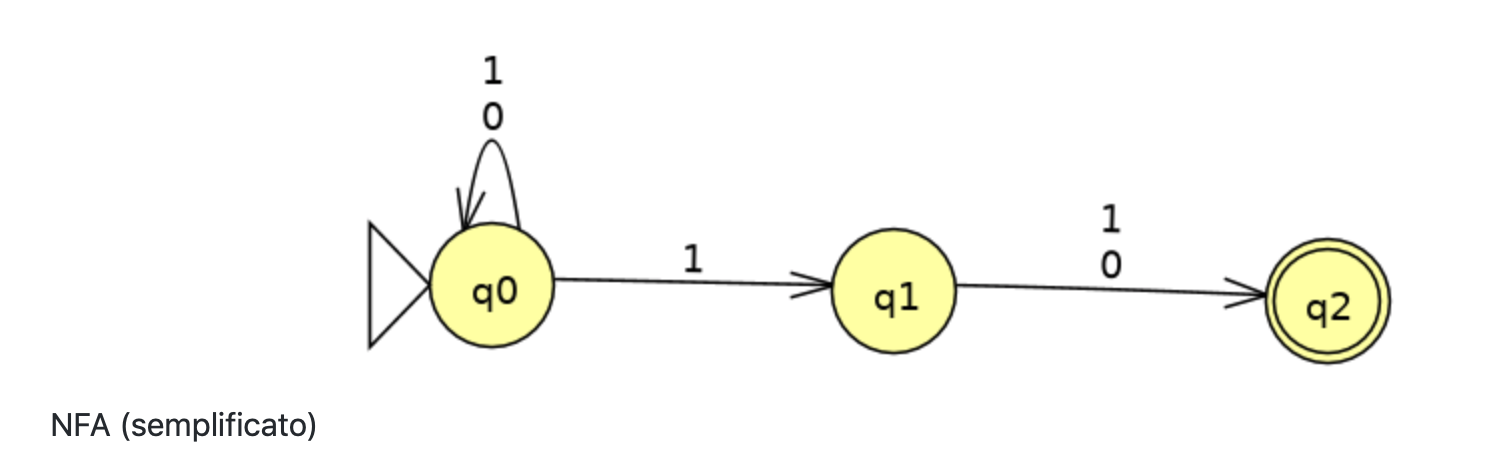
\includegraphics[width=5cm]{Lez2retodfa2.png}
        \end{minipage}
        \item \begin{minipage}{\linewidth}
            \centering
            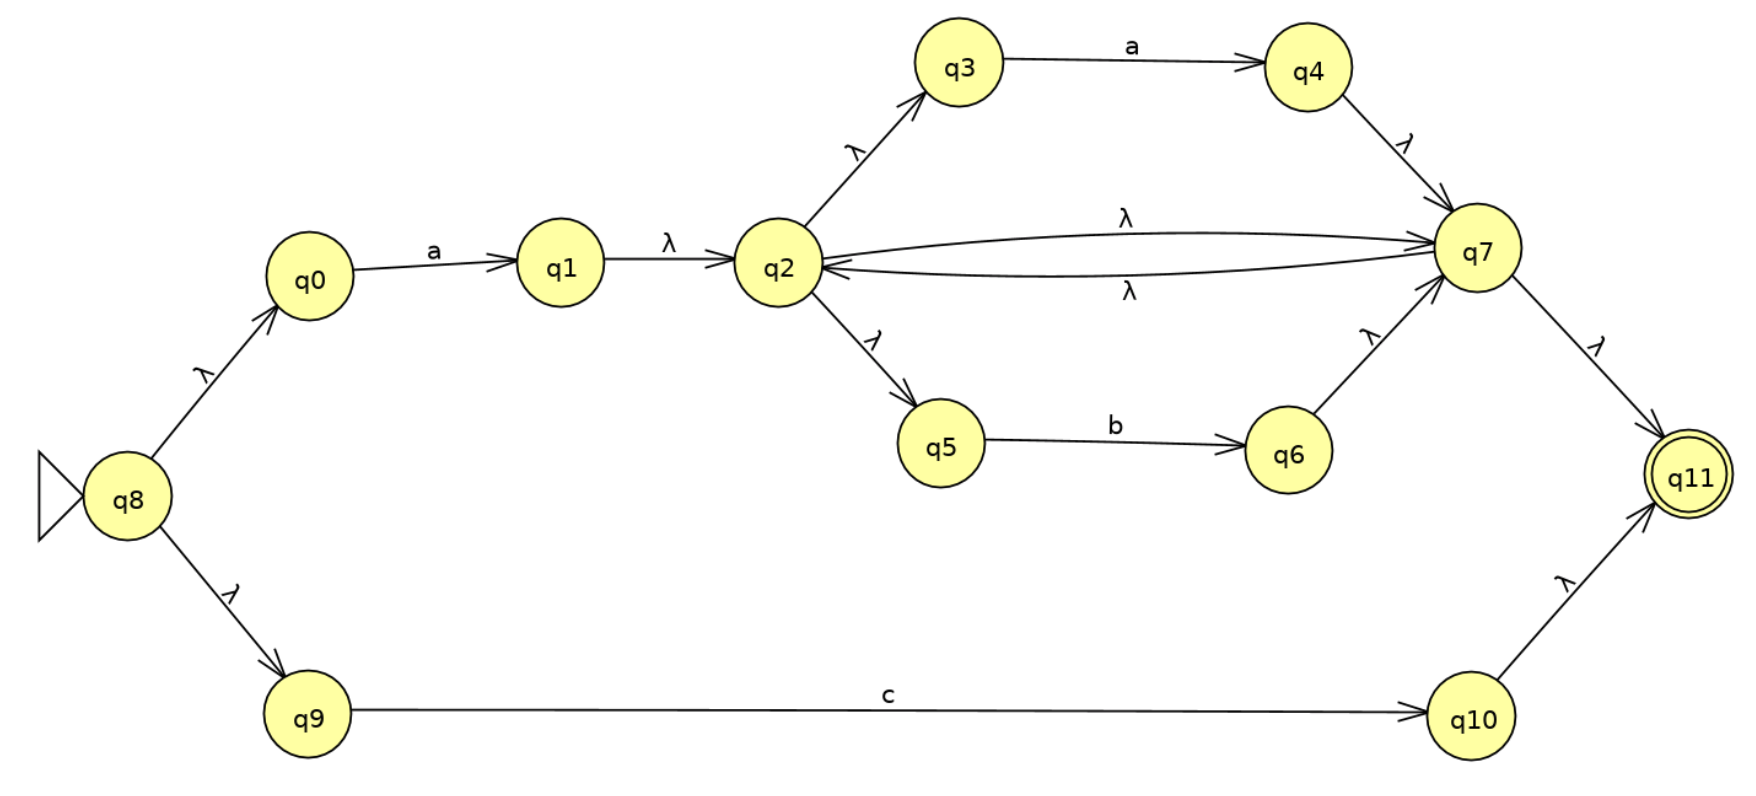
\includegraphics[width=5cm]{Lez2retodfa3.png}
        \end{minipage}
    \end{enumerate}
    Conversione da FA a RE
    \begin{enumerate}
        \item $R=(1+0((0+10^*1)1)^*(0+10^*1)0)^*$
        \item $R=((\epsilon+aa(aa)^*)ab)*(a+aa(aa)^*(\epsilon+a))$
    \end{enumerate}
    Dire se il linguaggio dato è regolare.
    \begin{enumerate}
        \item una regexp che riconosce lo stesso linguaggio è: $R=(00000)^*$. Supponendo che la regexp sia corretta possiamo dire che il linguaggio è regolare.
        \item a lezione è stato visto che $L_p=\{0^p,$ p è primo $\}$ è non regolare. Notiamo che $L=comp(L_p)$, quindi $L$ non è regolare poiché i linguaggi regolari sono chiusi per complementazione. Infatti:\\$L$ è regolare $\Rightarrow$ $comp(L)$ è regolare\\
        \begin{minipage}{\linewidth}
        \centering $\Leftrightarrow$ 
        \end{minipage}
        \\$comp(L)$ è non regolare $\Rightarrow$ $L$ è non regolare;
        \item Supponiamo per assurdo che L sia regolare. Allora vale il PL e sia h la lunghezza data dal PL;\
        Cerchiamo una parola $w\in L$ tale che $|w|\geq h$.\\
        Scegliamo $w=0^{h^3}$, che ovviamente soddisfa $|w|\geq h, \forall h \in \mathbb{N}$.\\
        Sia $w=xyz$ e $|xy|\leq h$, $y\neq\epsilon$. Allora $xy$ sarà fatta solo di $0$, cioè $x=0^n, y=0^m, n+m\leq h, m>0$.\\
        Proviamo a pompare y. Prendiamo $w^{'}=xy^2z=0^{h^3+m}$.\\Sono sufficienti per arrivare al cubo successivo? Alla meglio si ha $m=h$, ma si dimostra immediatamente che $(h+1)^3>h^3+h$. Quindi non basta (anche nel migliore dei casi), cioè $w'\notin L$ e quindi $L$ non è regolare.
        NB: formalmente si può dimostrare che $h^3<h^3+m\leq h^3+h<(h+1)^3$.
    \end{enumerate}
    % Bibliografia
    %\begin{thebibliography}{9}
        %  Alcune soluzio
    %\end{thebibliography}
    \end{document}